\documentclass[11pt,a4paper]{article}
\usepackage[T1]{fontenc}
\usepackage{lmodern}
\usepackage[top=0.48in, bottom=0.48in, left=0.68in, right=0.68in, headheight=0pt, headsep=0pt]{geometry}
\usepackage{amsmath,amssymb}
\usepackage{xcolor}
\usepackage{tikz}
\usetikzlibrary{arrows.meta,positioning,calc,decorations.pathreplacing}
\usepackage{tcolorbox}
\usepackage{hyperref}
\usepackage{booktabs}
\usepackage{url}
\usepackage{caption}

\hypersetup{
    colorlinks=true,
    linkcolor=blue!70!black,
    citecolor=blue!70!black,
    urlcolor=blue!70!black
}

% Custom Callout Boxes matching math_tools_en / house style
\newtcolorbox{learningobj}{
    colback=blue!3!white,
    colframe=blue!60!black,
    fonttitle=\bfseries\sffamily,
    fontupper=\small,
    title={$\blacktriangleright$ LEARNING OBJECTIVE},
    arc=1.5mm,
    boxrule=0.8pt,
    left=3.5mm, right=3.5mm, top=1.2mm, bottom=1.2mm,
    before skip=1mm, after skip=1.5mm
}

\newtcolorbox{groundbreaking}{
    colback=teal!4!white,
    colframe=teal!60!black,
    fonttitle=\bfseries\sffamily,
    title={$\bigstar$ GROUNDBREAKING FINDING},
    arc=1.5mm,
    boxrule=0.8pt,
    left=3.5mm, right=3.5mm, top=1.8mm, bottom=1.8mm
}

\newtcolorbox{physicalinsight}{
    colback=yellow!6!white,
    colframe=orange!75!black,
    fonttitle=\bfseries\sffamily,
    title={$\blacktriangleright$ PHYSICAL INSIGHT},
    arc=1.5mm,
    boxrule=0.8pt,
    left=3.5mm, right=3.5mm, top=1.8mm, bottom=1.8mm
}

\newtcolorbox{misconceptionbox}[1]{
    colback=red!2!white,
    colframe=red!70!black,
    fonttitle=\bfseries\sffamily,
    title={$\triangle$ MISCONCEPTION BUSTER: #1},
    arc=1.5mm,
    boxrule=0.8pt,
    left=3.5mm, right=3.5mm, top=1.5mm, bottom=1.5mm
}

\renewcommand{\thefigure}{1.2\alph{figure}}

\begin{document}

% ============================================================================
% PAGE 1: Physics of Speech & Nyquist Sampling
% ============================================================================
\vspace*{-4mm}
\section*{1.2 The Streaming Audio Preprocessing Pipeline}
\vspace{-1.5mm}

\begin{learningobj}
Rather than treating the frontend as a recipe (frame $\to$ FFT $\to$ Mel $\to$ log), this section walks the physical packets that cross each boundary. We trace how an infinite air pressure wave is sampled, buffered, windowed, transformed, filtered, and compressed into deterministic feature frames, proving why on-chip memory layouts and pointer arithmetic must mirror the exact dimensions of the underlying acoustic tensors.
\end{learningobj}

In Section 1.1 we established that acoustic physics forbids batching ($B > 1 \implies \text{latency}$). Yet, digital signal processors and neural acoustic models cannot ingest an infinite analog wave directly. To extract linguistic representations from continuous air pressure, we must construct a hardware-software datapath that slices, conditions, and transforms the streaming audio with absolute temporal determinism.

This section follows the dataflow across the six standard transformations implemented in the reference pipeline \nolinkurl{chapter01/exp_01_streaming_audio_pipeline.py}: the raw waveform, the sliding ring buffer, the tapering window, the Short-Time Fourier Transform (STFT), the Mel filterbank, and logarithmic compression. These stages do not form an arbitrary software syllabus. Each layer arises because the physical stage immediately preceding it leaves an unresolved mechanical dilemma that prevents the next arithmetic operation from executing:

{\small
\begin{itemize}\setlength{\itemsep}{-1.5pt}\setlength{\parsep}{0pt}\setlength{\topsep}{0.5pt}\setlength{\partopsep}{0pt}
    \item Air pressure is continuous, whereas digital hardware stores discrete numbers; the physical wave must therefore be \textbf{sampled} at uniform clock intervals.
    \item The streaming audio has no end, whereas frequency analysis requires a stationary, finite block of numbers; the system must therefore maintain a fixed-size \textbf{buffer} that steps forward by a discrete hop.
    \item Slicing an ongoing wave creates abrupt discontinuities at the frame boundaries, which a Fourier analyzer misinterprets as spurious high-frequency harmonics; each frame must therefore be \textbf{windowed} (tapered toward zero) before transformation.
    \item Tapering the frame edges suppresses boundary energy where acoustic information resides; consecutive frames must therefore \textbf{overlap heavily}, triggering a full spectral analysis once every hop rather than once per window length.
    \item A windowed frame remains in the time domain, hiding resonance frequencies; the \textbf{STFT} evaluates the frame against $N$ candidate probing frequencies to generate a spectral power representation.
    \item The resulting $257$ linear frequency bins are too redundant for downstream acoustic models and follow a linear Hertz scale that ignores human hearing; they are pooled into $80$ non-linear \textbf{Mel filterbank bands}.
    \item Energy values across spectral bands vary across multiple orders of magnitude, causing neural network additions to be dominated by the loudest band; each energy value is therefore compressed by taking its \textbf{logarithm}.
\end{itemize}
}

\vspace{0.5mm}
\hrule
\vspace{0.5mm}

\vspace{-2mm}
\subsection*{Step 1: The Waveform and Nyquist Sampling}
\vspace{-1.5mm}

Sound is recorded as a discrete time-series measuring fluctuations in atmospheric air pressure. The temporal spacing between measurements is dictated by the \textbf{sampling frequency} ($f_s$), defining the number of discrete samples captured per second.

The standard edge voice pipeline operates at $f_s = 16\text{ kHz}$. Every $T_s = 62.5\,\mu\text{s}$, exactly one new sample emerges from the microphone analog-to-digital converter (ADC), and a $25\text{ ms}$ analysis window accumulates $400$ samples. This parameter choice is rooted in the biomechanics of human vocal production:
\begin{itemize}\setlength{\itemsep}{-1pt}\setlength{\parsep}{0pt}\setlength{\topsep}{0.5pt}\setlength{\partopsep}{0pt}
    \item The vocal folds vibrate at a fundamental frequency ($F_0$) ranging from $85\text{ Hz}$ (deep male voice) to $255\text{ Hz}$ (high female voice).
    \item The resonant cavities of the vocal tract (pharynx, oral cavity, and nasal cavity) generate formant peaks ($F_1, F_2, F_3$) that define vowel identities, spanning from $300\text{ Hz}$ to $3{,}500\text{ Hz}$.
    \item The highest acoustic frequencies in human speech occur during voiceless fricatives and plosives (such as /s/ and /sh/), which decay rapidly above $8\text{ kHz}$.
\end{itemize}

According to the Nyquist-Shannon sampling theorem, perfect reconstruction of a band-limited signal requires a sampling frequency at least twice its highest frequency component ($f_s \ge 2B$). A sampling rate of $16\text{ kHz}$ places the Nyquist boundary at $8\text{ kHz}$, encapsulating the entire human phonetic spectrum while rejecting ultrasonic ambient noise. Raising the rate to the CD standard ($44.1\text{ kHz}$) or studio standard ($48\text{ kHz}$) triples the on-chip buffer size, bus bandwidth, and arithmetic compute load without contributing any meaningful phonetic information to the acoustic model.

\clearpage

\subsection*{Step 2: The Sliding Ring Buffer}

The front end observes a window of $L = 400$ samples every hop, advancing across the input stream in strides of $H = 160$ samples ($T_h = 10\text{ ms}$).

To understand how hardware resolves this overlap, consider two competing implementation hypotheses:

\begin{itemize}\setlength{\itemsep}{1pt}\setlength{\parskip}{0pt}
    \item \textbf{Hypothesis A (The Naive Software Shift):} The processor treats the frame buffer as a contiguous linear array. When $160$ new samples arrive, the software executes a memory shift (\texttt{memmove}), copying the most recent $240$ samples downward to the beginning of the buffer before appending the new $160$ samples at the tail.
    \item \textbf{Hypothesis B (The Hardware Circular Pointer Buffer):} The memory addresses remain fixed in silicon storage. Instead of moving data elements, the architecture updates two circular address pointers that increment modulo $400$.
\end{itemize}

The resolution demonstrates the efficiency of custom hardware over general-purpose memory buses: under Hypothesis A, the processor pays a recurring memory traffic tax on every frame ($240$ reads and $240$ writes). Under Hypothesis B, the physical samples never move once written to Block RAM (BRAM). The write pointer advances by $160$ addresses to overwrite the oldest data, while the read pointer streams $400$ contiguous samples into the computation datapath starting from the updated boundary.

\begin{center}\vspace{-2mm}
\begin{minipage}{\textwidth}
\centering
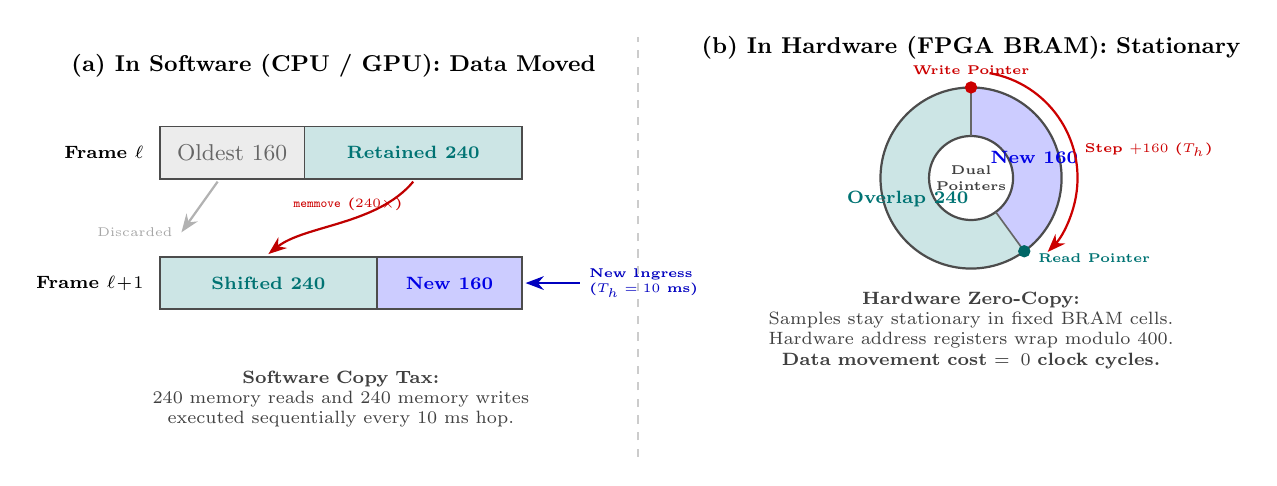
\begin{tikzpicture}[
  >=Stealth,
  scale=0.92, every node/.style={transform shape},
  font=\small,
  blk/.style={draw=black!70, semithick, align=center, inner sep=2pt, minimum height=7.2mm},
  oldblk/.style={blk, fill=gray!15, text=black!60},
  ovrblk/.style={blk, fill=teal!20, text=teal!90!black, font=\scriptsize\bfseries},
  newblk/.style={blk, fill=blue!20, text=blue!90!black, font=\scriptsize\bfseries},
  ann/.style={font=\scriptsize, text=black!75, align=center},
  ttl/.style={font=\bfseries\small, align=left}
]

% ==================== (a) SOFTWARE: Data is Copied ====================
\node[ttl] at (2.4, 4.8) {(a) In Software (CPU / GPU): Data Moved};

% Frame l
\node[font=\scriptsize\bfseries, anchor=east] at (-0.1, 3.6) {Frame $\ell$};
\node[oldblk, minimum width=2.0cm] at (1.0, 3.6) {Oldest 160};
\node[ovrblk, minimum width=3.0cm] at (3.5, 3.6) {Retained 240};

% Frame l+1
\node[font=\scriptsize\bfseries, anchor=east] at (-0.1, 1.8) {Frame $\ell\!+\!1$};
\node[ovrblk, minimum width=3.0cm] at (1.5, 1.8) {Shifted 240};
\node[newblk, minimum width=2.0cm] at (4.0, 1.8) {New 160};

% Shift arrow
\draw[thick, ->, red!75!black] (3.5, 3.2) .. controls (3.0, 2.6) and (2.0, 2.6) .. (1.5, 2.2);
\node[font=\tiny\bfseries, text=red!80!black, above=2pt] at (2.6, 2.6) {\texttt{memmove} ($240\times$)};

% Discard arrow
\draw[->, gray!60, thick] (0.8, 3.2) -- (0.3, 2.5);
\node[font=\tiny, text=gray!70, left] at (0.3, 2.5) {Discarded};

% Ingress arrow
\draw[->, blue!75!black, thick] (5.8, 1.8) node[right, font=\tiny\bfseries, align=left] {New Ingress\\($T_h = 10\text{ ms}$)} -- (5.05, 1.8);

\node[ann, text width=5.6cm] at (2.5, 0.2) {
  \textbf{Software Copy Tax:}\\
  $240$ memory reads and $240$ memory writes executed sequentially every $10\text{ ms}$ hop.
};

% ==================== DIVIDER ====================
\draw[dashed, gray!40, thick] (6.6, -0.6) -- (6.6, 5.2);

% ==================== (b) HARDWARE: Circular BRAM ====================
\begin{scope}[shift={(11.2, 2.6)}]
  \node[ttl, align=center] at (0, 2.45) {(b) In Hardware (FPGA BRAM): Stationary};

  \def\R{1.25}\def\ri{0.58}
  \def\cy{0.65}
  % 160 samples = 144 deg (from 90 to -54)
  % 240 samples = 216 deg (from -54 to -270)
  \fill[blue!20] (0,\cy) -- ++(90:\R) arc (90:-54:\R) -- cycle;
  \fill[teal!20] (0,\cy) -- ++(-54:\R) arc (-54:-270:\R) -- cycle;
  \fill[white] (0,\cy) circle (\ri);

  \draw[black!70, thick] (0,\cy) ++(90:\R) arc (90:-270:\R);
  \draw[black!70, thick] (0,\cy) ++(90:\ri) arc (90:-270:\ri);
  \draw[black!60, semithick] (0,\cy) ++(90:\ri) -- ++(90:\R-\ri);
  \draw[black!60, semithick] (0,\cy) ++(-54:\ri) -- ++(-54:\R-\ri);

  \node[font=\scriptsize\bfseries, text=blue!90!black] at ($(0,\cy)+(18:0.92)$) {New 160};
  \node[font=\scriptsize\bfseries, text=teal!90!black] at ($(0,\cy)+(-162:0.92)$) {Overlap 240};

  % Write Pointer
  \filldraw[red!80!black] ($(0,\cy)+(90:\R)$) circle (2.2pt);
  \node[font=\tiny\bfseries, text=red!80!black, anchor=south] at ($(0,\cy)+(90:\R+0.05)$) {Write Pointer};
  \draw[thick, ->, red!80!black] ($(0,\cy)+(80:\R+0.22)$) arc (80:-44:\R+0.22);
  \node[font=\tiny\bfseries, text=red!80!black, right] at ($(0,\cy)+(15:\R+0.25)$) {Step $+160$ ($T_h$)};

  % Read Pointer (at -54 deg, label to the right)
  \filldraw[teal!80!black] ($(0,\cy)+(-54:\R)$) circle (2.2pt);
  \node[font=\tiny\bfseries, text=teal!90!black, anchor=west] at ($(0,\cy)+(-54:\R+0.12)$) {Read Pointer};

  % Center text
  \node[font=\tiny\bfseries, text=black!75, align=center] at (0,\cy) {Dual\\Pointers};

  \node[ann, text width=6.2cm] at (0, -1.45) {
    \textbf{Hardware Zero-Copy:}\\
    Samples stay stationary in fixed BRAM cells.\\
    Hardware address registers wrap modulo $400$.\\
    \textbf{Data movement cost $= 0$ clock cycles.}
  };
\end{scope}

\end{tikzpicture}\\[2mm]
\refstepcounter{figure}\label{fig:1_2a_ring_buffer}
\begin{minipage}{0.95\textwidth}
\small\textbf{Figure \thefigure}: The mechanical contrast between software memory shifting and hardware circular ring buffering for a 400-sample window with a 160-sample hop ($T_h = 10\text{ ms}$). Notice that while software moves 240 samples per frame via sequential reads and writes, the hardware architecture stores audio in fixed on-chip Block RAM cells and advances dual address registers modulo 400. This proves that dedicated FPGA storage eliminates data movement overhead entirely, reducing data transfer cost to zero clock cycles.
\end{minipage}
\end{minipage}\vspace{-2mm}
\end{center}

\begin{groundbreaking}
On spatial FPGA architectures, data movement cost for frame overlap drops to zero:
$$\text{Data Movement Energy} \to 0$$
Inter-frame acoustic state does not live in software copy loops. It lives entirely in the address bits of circular BRAM pointer registers. This circular buffer forms the first persistent state module in the streaming voice pipeline.
\end{groundbreaking}

\clearpage

\subsection*{Step 3: Windowing and the Boundary Discontinuity}

A 400-sample analysis window represents a finite rectangular cut extracted from an ongoing analog sound wave. A rectangular truncation acts as a sharp step function: the signal starts instantaneously at sample $0$ and cuts off abruptly at sample $399$.

To a Fourier analyzer, an instantaneous vertical transition cannot be distinguished from high-frequency harmonics that never existed in the acoustic environment. If transformed directly, these boundary cliffs produce severe \textbf{spectral leakage}, smearing energy across adjacent frequency bins.

To prevent this distortion, the 400 samples stored in the ring buffer are multiplied element-wise by a symmetric \textbf{Hamming window} $w[n]$:
$$x_w[n] = x[n] \cdot w[n], \quad 0 \le n < 400$$

The Hamming window tapers smoothly toward near-zero at both margins, ensuring that the waveform enters and exits the analysis frame without sharp step transitions.

\begin{physicalinsight}
A tapering window is a boundary tax paid so that the Fourier analyzer does not encounter an artificial cliff. By forcing the boundary samples toward zero, the window suppresses spurious high-frequency harmonics at the cost of attenuating real edge energy. This attenuation causes spectral broadening, which is why consecutive frames must overlap heavily by $240$ samples to ensure every acoustic event is analyzed near a window peak.
\end{physicalinsight}

\smallskip
\hrule
\smallskip

\subsection*{Step 4: The Short-Time Fourier Transform (STFT)}

Computing the Discrete Fourier Transform (DFT) on consecutive windowed frames across time forms the Short-Time Fourier Transform (STFT). 

To compute the DFT efficiently, the 400 windowed samples are extended to $512$ samples by appending $112$ zero values (\textbf{zero-padding}). Padding to a power of two ($N_{\text{fft}} = 512$) enables the use of radix-2 Fast Fourier Transform (FFT) pipelines.

Because the incoming audio signal consists entirely of real-valued numbers, the resulting complex spectrum possesses Hermitian symmetry: the upper half of the frequency bins is a redundant conjugate mirror of the lower half. The engine discards the redundant negative frequencies, retaining only the $N_{\text{fft}} / 2 + 1 = 257$ non-redundant positive frequency bins. Taking the squared magnitude of these complex values yields the power spectrum:
$$P[k] = |X[k]|^2, \quad 0 \le k \le 256$$

\smallskip
\hrule
\smallskip

\subsection*{Step 5: The Mel Filterbank}

The $257$ linear power spectrum bins provide uniform frequency resolution across the entire $0\text{ to }8\text{ kHz}$ range ($8{,}000 / 256 = 31.25\text{ Hz}$ per bin). 

However, human auditory perception does not perceive frequency differences on a linear scale. The human cochlea resolves low-frequency tones with high precision while grouping high-frequency tones into broad perceptual bands. Furthermore, feeding $257$ raw spectral values directly into a small neural network inflates the parameter count unnecessarily.

The pipeline compresses the $257$ linear bins into $M = 80$ \textbf{Mel filterbank bands}. Each Mel filter is a triangular weighting function spanning a cluster of adjacent FFT bins. Filters are densely spaced at low frequencies and widen progressively at higher frequencies. The output energy $E[m]$ for the $m$-th Mel band is computed as the weighted sum of the linear power spectrum bins overlapping that filter:
$$E[m] = \sum_{k=0}^{256} W[m, k] \cdot P[k], \quad 0 \le m < 80$$
where $W$ is the precomputed $80 \times 257$ sparse triangular weighting matrix.

\clearpage

\subsection*{Step 6: Logarithmic Compression}

Acoustic energy across the $80$ Mel bands can vary by factors of millions between soft vocal murmurs and loud plosive bursts. If raw energy values were fed directly into a neural acoustic model, large amplitudes would saturate activation functions and dominate gradient updates.

Furthermore, human perception of loudness conforms to the Weber-Fechner law: the perceived increase in volume is proportional to the ratio of sound intensity rather than absolute linear differences.

The final preprocessing stage compresses each Mel energy band logarithmically:
$$S[m] = \ln\left(\max\left(E[m], \, 10^{-6}\right)\right), \quad 0 \le m < 80$$

The floor threshold of $10^{-6}$ serves a critical arithmetic purpose: during periods of absolute silence where band energy approaches zero, the clamp prevents the logarithmic operator from evaluating to negative infinity ($-\infty$), guaranteeing numerical stability in fixed-point and floating-point hardware pipelines.

\smallskip
\hrule
\smallskip

\subsection*{Tensor Dimensions and Memory Footprint}

In silicon architectures, tensor dimensions are not abstract software dimensions; they dictate register bit-widths, Block RAM depth, and memory bus bandwidth. The complete data progression across a single $10\text{ ms}$ frame is summarized in Table~\ref{tab:tensor_sizes}:

\begin{center}\vspace{-1mm}
\begin{minipage}{\textwidth}
\centering
\small
\captionof{table}{Streaming audio tensor dimensions and FP32 memory sizes per $10\text{ ms}$ frame.}\label{tab:tensor_sizes}
\vspace{1mm}
\begin{tabular}{lll}
\toprule
\textbf{Processing Layer} & \textbf{Data Produced per Frame} & \textbf{FP32 Footprint (Float 32-bit)} \\
\midrule
Incoming Waveform & 160 new samples & 640 B loaded every $10\text{ ms}$ \\
Sliding Ring Buffer & 400 resident samples & 1,600 B, persistent on-chip state \\
Windowed Frame & 400 windowed samples & 1,600 B (buffer $\times$ Hamming window) \\
FFT Input Buffer & 512 samples & 2,048 B (400 real samples $+ 112$ zero-pad) \\
Power Spectrum & 257 spectral bins & 1,028 B (257 real energy values) \\
Mel Filterbank Bands & 80 filterbank values & 320 B ($80 \times 257$ matrix multiply) \\
Log-Mel Feature Frame & 80 log-energy features & 320 B (direct input to acoustic model) \\
\bottomrule
\end{tabular}
\end{minipage}
\end{center}

\begin{center}\vspace{-2mm}
\begin{minipage}{\textwidth}
\centering
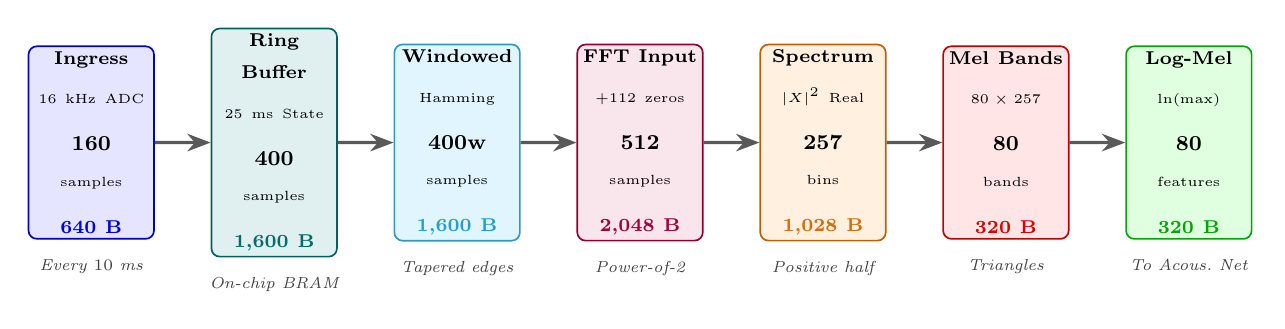
\begin{tikzpicture}[
  >=Stealth,
  scale=0.96, every node/.style={transform shape},
  tensor/.style={
    draw=black!75, rounded corners=3pt, semithick, align=center,
    inner sep=2pt, minimum height=21mm, text width=1.52cm
  },
  t1/.style={tensor, fill=blue!10, draw=blue!75!black},
  t2/.style={tensor, fill=teal!12, draw=teal!75!black},
  t3/.style={tensor, fill=cyan!12, draw=cyan!75!black},
  t4/.style={tensor, fill=purple!10, draw=purple!75!black},
  t5/.style={tensor, fill=orange!12, draw=orange!75!black},
  t6/.style={tensor, fill=red!10, draw=red!75!black},
  t7/.style={tensor, fill=green!12, draw=green!65!black},
  arrow/.style={->, very thick, black!65}
]

\def\xdist{2.42}

% Stage 1: 160
\node[t1] (s1) at (0*\xdist, 0) {
  {\fontsize{7}{8}\selectfont\bfseries Ingress}\\[1mm]
  {\fontsize{5.5}{6.5}\selectfont $16\text{ kHz}$ ADC}\\[2mm]
  {\fontsize{8}{9}\selectfont\bfseries 160}\\[0.5mm]
  {\fontsize{5.5}{6.5}\selectfont samples}\\[2mm]
  {\fontsize{7}{8}\selectfont\bfseries\color{blue!85!black} 640 B}
};

% Stage 2: 400
\node[t2] (s2) at (1*\xdist, 0) {
  {\fontsize{7}{8}\selectfont\bfseries Ring Buffer}\\[1mm]
  {\fontsize{5.5}{6.5}\selectfont $25\text{ ms}$ State}\\[2mm]
  {\fontsize{8}{9}\selectfont\bfseries 400}\\[0.5mm]
  {\fontsize{5.5}{6.5}\selectfont samples}\\[2mm]
  {\fontsize{7}{8}\selectfont\bfseries\color{teal!85!black} 1,600 B}
};

% Stage 3: 400w
\node[t3] (s3) at (2*\xdist, 0) {
  {\fontsize{7}{8}\selectfont\bfseries Windowed}\\[1mm]
  {\fontsize{5.5}{6.5}\selectfont Hamming}\\[2mm]
  {\fontsize{8}{9}\selectfont\bfseries 400w}\\[0.5mm]
  {\fontsize{5.5}{6.5}\selectfont samples}\\[2mm]
  {\fontsize{7}{8}\selectfont\bfseries\color{cyan!85!black} 1,600 B}
};

% Stage 4: 512
\node[t4] (s4) at (3*\xdist, 0) {
  {\fontsize{7}{8}\selectfont\bfseries FFT Input}\\[1mm]
  {\fontsize{5.5}{6.5}\selectfont $+112$ zeros}\\[2mm]
  {\fontsize{8}{9}\selectfont\bfseries 512}\\[0.5mm]
  {\fontsize{5.5}{6.5}\selectfont samples}\\[2mm]
  {\fontsize{7}{8}\selectfont\bfseries\color{purple!85!black} 2,048 B}
};

% Stage 5: 257
\node[t5] (s5) at (4*\xdist, 0) {
  {\fontsize{7}{8}\selectfont\bfseries Spectrum}\\[1mm]
  {\fontsize{5.5}{6.5}\selectfont $|X|^2$ Real}\\[2mm]
  {\fontsize{8}{9}\selectfont\bfseries 257}\\[0.5mm]
  {\fontsize{5.5}{6.5}\selectfont bins}\\[2mm]
  {\fontsize{7}{8}\selectfont\bfseries\color{orange!85!black} 1,028 B}
};

% Stage 6: 80
\node[t6] (s6) at (5*\xdist, 0) {
  {\fontsize{7}{8}\selectfont\bfseries Mel Bands}\\[1mm]
  {\fontsize{5.5}{6.5}\selectfont $80\times 257$}\\[2mm]
  {\fontsize{8}{9}\selectfont\bfseries 80}\\[0.5mm]
  {\fontsize{5.5}{6.5}\selectfont bands}\\[2mm]
  {\fontsize{7}{8}\selectfont\bfseries\color{red!85!black} 320 B}
};

% Stage 7: 80 log
\node[t7] (s7) at (6*\xdist, 0) {
  {\fontsize{7}{8}\selectfont\bfseries Log-Mel}\\[1mm]
  {\fontsize{5.5}{6.5}\selectfont $\ln(\max)$}\\[2mm]
  {\fontsize{8}{9}\selectfont\bfseries 80}\\[0.5mm]
  {\fontsize{5.5}{6.5}\selectfont features}\\[2mm]
  {\fontsize{7}{8}\selectfont\bfseries\color{green!65!black} 320 B}
};

% Connecting Arrows
\draw[arrow] (s1) -- (s2);
\draw[arrow] (s2) -- (s3);
\draw[arrow] (s3) -- (s4);
\draw[arrow] (s4) -- (s5);
\draw[arrow] (s5) -- (s6);
\draw[arrow] (s6) -- (s7);

% Bottom notes
\node[font=\fontsize{6.5}{7.5}\selectfont\itshape, text=black!75, below=4pt of s1] {Every $10\text{ ms}$};
\node[font=\fontsize{6.5}{7.5}\selectfont\itshape, text=black!75, below=4pt of s2] {On-chip BRAM};
\node[font=\fontsize{6.5}{7.5}\selectfont\itshape, text=black!75, below=4pt of s3] {Tapered edges};
\node[font=\fontsize{6.5}{7.5}\selectfont\itshape, text=black!75, below=4pt of s4] {Power-of-2};
\node[font=\fontsize{6.5}{7.5}\selectfont\itshape, text=black!75, below=4pt of s5] {Positive half};
\node[font=\fontsize{6.5}{7.5}\selectfont\itshape, text=black!75, below=4pt of s6] {Triangles};
\node[font=\fontsize{6.5}{7.5}\selectfont\itshape, text=black!75, below=4pt of s7] {To Acous.~Net};

\end{tikzpicture}\\[2mm]
\refstepcounter{figure}\label{fig:1_2b_pipeline_tensor_sizes}
\begin{minipage}{0.95\textwidth}
\small\textbf{Figure \thefigure}: Tensor dimensions and memory footprint along the streaming audio datapath for one 10 ms analysis frame. Notice how the data representation expands from 160 samples (640 B) to 512 zero-padded points (2,048 B) for spectral computation, then compresses down to 80 compact log-energy values (320 B) for neural network inference. This proves that hardware buffer sizing and bus widths are directly dictated by the mathematical tensor shapes of the DSP pipeline.
\end{minipage}
\end{minipage}\vspace{-2mm}
\end{center}
\clearpage

\subsection*{Misconception Buster: Three Traps in Streaming Voice Preprocessing}

The following cognitive traps frequently mislead developers transitioning from offline machine learning or general-purpose computing to edge FPGA implementation:

\begin{misconceptionbox}{Trap A --- Higher Sampling Rate ($48\text{ kHz}$) Improves AI Accuracy}
\textbf{Root Cause:} Hi-fi audio intuition conflates higher sampling rates ($48\text{ kHz}$ or $96\text{ kHz}$) with crisper musical reproduction, leading developers to assume higher rates increase acoustic model accuracy.\\[1mm]
\textbf{Scientific Reality:} Human speech formants ($F_1, F_2, F_3$) reside between $300\text{ Hz}$ and $3{,}500\text{ Hz}$, while voiceless fricatives decay before $8\text{ kHz}$. Raising $f_s$ to $48\text{ kHz}$ captures only ambient ultrasonic hiss while tripling on-chip BRAM allocation, bus bandwidth, and FFT arithmetic complexity, offering zero phonetic advantage to the acoustic model.
\end{misconceptionbox}

\begin{misconceptionbox}{Trap B --- The Sliding Frame Buffer Is Merely a Software Memory Copy}
\textbf{Root Cause:} In standard Python or C implementations, stepping the analysis frame is executed using memory shift routines (\texttt{memmove}), requiring $240$ read and $240$ write cycles on every hop.\\[1mm]
\textbf{Scientific Reality:} On spatial FPGA hardware, a circular buffer consumes zero copy clock cycles. By implementing two hardware counter registers that cycle around on-chip Block RAM, audio samples remain stationary while addresses wrap modulo 400. The sequential $\mathcal{O}(L-H)$ memory transfer overhead disappears entirely.
\end{misconceptionbox}

\begin{misconceptionbox}{Trap C --- Rectangular Window Slicing Preserves Unaltered Audio Samples}
\textbf{Root Cause:} A flat rectangular cut preserves the exact numerical values of raw audio samples without multiplying by scaling coefficients, creating the illusion of perfect signal fidelity.\\[1mm]
\textbf{Scientific Reality:} Sharp step discontinuities at frame boundaries generate spurious high-frequency harmonics absent from the recording room. To a Fourier transform, sudden edges resemble infinite-frequency impulses that cause severe spectral leakage across adjacent bins. Applying a smooth tapering window (Hamming) is physically mandatory to eliminate boundary artifacts.
\end{misconceptionbox}

\smallskip
\hrule
\smallskip

\subsection*{The Unresolved Dilemma: The Frequency Blur}

Through the six stages of this pipeline, we have successfully conditioned raw air pressure waves into stationary 80-dimensional feature vectors emitted once every $10\text{ ms}$. 

Yet, this transformation reveals a fundamental physical tension: when we squeezed the analysis window down to $25\text{ ms}$ to preserve temporal stationarity, what happened to our ability to distinguish two closely spaced resonance frequencies? Why does an FFT bin spanning $31.25\text{ Hz}$ blur adjacent harmonics, and how does the Mel filterbank balance this trade-off between time resolution and frequency resolution?

This mathematical dilemma brings us directly to the formal derivation of the STFT and Mel filterbank in Section 1.3.

\end{document}
